%!TEX encoding = UTF-8 Unicode
\documentclass[11pt,a4paper,papersize,oneside]{jsbook}

\usepackage[OT2,T1]{fontenc}
\usepackage{amsmath}
\usepackage{amssymb}
\usepackage{newtxtext,newtxmath}
\usepackage[dvipdfmx]{graphicx}
\graphicspath{{Fig/}}
\usepackage{url}
\usepackage[dvipdfmx]{hyperref}
\usepackage[dvipdfmx]{pxjahyper} % 日本語のhyperref
\usepackage{makeidx}\makeindex  % allows for indexgeneration

\usepackage{pifont}
\usepackage{array,booktabs}
\usepackage{setspace}
\usepackage{enumitem}

% PDF meta information and bookmarks
\hypersetup{
bookmarks=true,         % show bookmarks bar?
bookmarksnumbered=true,
bookmarkstype=toc,
%unicode=true,          % non-Latin characters in Acrobat’s bookmarks
pdftoolbar=true,        % show Acrobat’s toolbar?
pdfmenubar=true,        % show Acrobat’s menu?
pdffitwindow=false,     % window fit to page when opened
pdftitle={推薦システムのアルゴリズム},    % title
pdfauthor={神嶌 敏弘},     % author
pdfsubject={}, % subject
pdfkeywords={推薦システム;recommender system;協調フィルタリング;collaborative filtering}, % list of keywords
pdfnewwindow=true,      % links in new window
%setpagesize=false, % setting paper size
}

% local macro definitions
\usepackage{mathsymbols}
\usepackage{myindex}

% set pagesize: A4paper, margin=3cm
\setlength{\topmargin}{4.6truemm}
\setlength{\headheight}{1\baselineskip}
\setlength{\headsep}{1\baselineskip}
\setlength{\textheight}{\paperheight}\addtolength{\textheight}{-60truemm}\addtolength{\textheight}{-2\baselineskip}
\setlength{\footskip}{0pt}
\setlength{\oddsidemargin}{4.6truemm}
\setlength{\evensidemargin}{\oddsidemargin}
\setlength{\textwidth}{\paperwidth}\addtolength{\textwidth}{-60truemm}
\setlength{\fullwidth}{\textwidth}

%%%% more linebreaks in equations %%%%

\binoppenalty=0
\relpenalty=0
% \mathcode`\,="202C      % "," is considered as a binary operator

%%%%% condense floats %%%%%

%\def\topfraction{0.99}
%\def\bottomfraction{0.01}
%\def\textfraction{0.01}
%\def\floatpagefraction{0.99}
%\def\dbltopfraction{0.99}
%\def\dblfloatpagefraction{0.99}

%%%%% title, author, and release %%%%%

\title{\LARGE\textbf{推薦システムのアルゴリズム}}
\author{\textbf{神嶌 敏弘}\quad$\langle$\url{http://www.kamishima.net/}$\rangle$}
\date{Release: \input{version}}

\begin{document}

% ===== Front Matter =====
\frontmatter

% --- Title ---
\maketitle

% --- Preface & Notation---
\onehalfspacing

%!TEX root =  main.tex
%!TEX encoding = UTF-8 Unicode
\chapter*{まえがき}
\label{chap:preface}

本稿は推薦システムについてまとめたものである.

人工知能学会誌2007年11月号~\cite{jpublist:076},2008年1月号~\cite{jpublist:081},および2008年3月号~\cite{jpublist:083}の3回に渡って連載した解説記事「推薦システムのアルゴリズム(1)〜(3)」に対し,誤りの訂正や,新しい内容の追加などの更新を行ったものである.

本稿のソースファイルは \texttt{GitHub} にて公開している.
\begin{quote}
\url{https://github.com/tkamishima/recsysdoc}
\end{quote}
TYPOや記述の誤りなどのバグリポートは,\texttt{GitHub} の rull request か,issues を使って連絡されたい.
なお,事情によりすぐには対処できない場合があるので,予めご了解いただきたい.

\section*{本稿の構成}
\label{sec:preface-organization}

本稿の構成は以下のとおりである.
第\ref{part:overview}部では,推薦システムとは何か,またその設計指針や分類について述べる.
第\ref{part:process}部では,データの入力,嗜好の予測,そして推薦の提示からなる推薦システムの実行過程について述べる.
第\ref{part:algoirthm}部では,さまざまな嗜好の予測アルゴリズムのを紹介する.
第\ref{part:topic}部では,推薦システムに関連する話題や,さまざまな状況での推薦を紹介する.
第\ref{part:conclusion}部は関連資料の紹介とまとめである.

%!TEX root =  main.tex
%!TEX encoding = UTF-8 Unicode
\chapter*{数式の表記}
\label{chap:notation}

スカラーの変数はイタリック体 $x$ で,一部の確立変数は大文字のイタリック体 $X$,ベクトルは小文字ボールド体 $\bfx$で,行列は大文字ボールド体 $\bfX$で表記する.
実数などの特殊なものを除き,集合にはカリグラフィック体 $\calD$ を用いる.

\begin{center}
\small\renewcommand{\arraystretch}{0.8}
\begin{tabular}{@{}>{\centering}p{0.09\fullwidth}@{\hspace{0.01\fullwidth}}p{0.38\fullwidth}@{\hspace{0.04\fullwidth}}>{\centering}p{0.09\fullwidth}@{\hspace{0.01\fullwidth}}p{0.38\textwidth}@{}}\toprule
\textbf{表記} & \textbf{意味} & \textbf{表記} & \textbf{意味} \\ \cmidrule(r){1-2}\cmidrule{3-4}
$x$ & 特定の利用者を表す & $y$ & 特定のアイテムを表す \\
$X$ & 利用者を表す確率変数 & $Y$ & アイテムを表す確率変数 \\
$\bfx$ & 利用者をまとめたベクトル & $\bfy$ & アイテムをまとめたベクトル \\
$n$ & 利用者数 & $m$ & アイテム数 \\
$\calX$ & 利用者集合 $\{1,\ldots,n\}$ & $\calY$ & アイテム集合 $\{1,\ldots,m\}$ \\
$\calX_y$ & アイテム$y$を評価した利用者の集合 & $\calY_x$ & 利用者xが評価したアイテムの集合 \\
$a$ & 活動利用者を表す & $r_{xy}$ & 利用者$x$のアイテム$y$への評価値 \\
$\bar{r}_x$ & 利用者$x$による評価値の平均 & $\tilde{r}_y$ & アイテム$y$への評価値の平均 \\
$\bfR$ & 評価値行列 & $\calR$ & 評価値集合(5段階評価なら $\{1,\ldots,5\}$) \\
$\bfr$ & 評価値をまとめたベクトル & $z$ & 潜在因子 \\
$\bfz$ & 潜在因子のベクトル & $K$ & 潜在因子の数・次元数 \\
$\calD$ & データ集合 & $N$ & 訓練データ数 \\
$\bfU$ & 利用者潜在因子行列 & $\bfV$ & アイテム潜在因子行列 \\
$\bfu_{x}$ & 利用者$x$の潜在因子ベクトル & $\bfv_{y}$ & アイテム$y$の潜在因子ベクトル \\
$y^{(t)}$ & 時刻$t$での値 & $\ang{Y^{(t)}}$ & アイテムの時系列 \\
$\theta\,\bftheta\,\bfTheta$ & パラメータを一般に表す & $\sig()$ & シグモイド関数 \\
$\Dom()$ & 変数の定義域 & $\nan$ & 欠損値 \\
\bottomrule
\end{tabular}
\end{center}

スカラー関数 $f(x)$ に対して,その引数をベクトルとする表記 $f(\bfx)$ は,ベクトル $\bfx$ の各要素を関数 $f$ に適用して得られるベクトルを表す.

確率変数 $X$ が離散の場合の確率質量関数も,連続値の場合の確率密度関数も特に区別することなく $\pb{X}$ と表記する.

$\expect_{\pb[X]}[f(X)]$ は,分布 $\pb{X}$ についての次の期待値を表す:
\[
\begin{array}{l@{\text{ \makebox[3zw]{\dotfill} }}l}
\sum_{x\in\Dom(X)} f(x) \pb{X=x} & \text{$X$が離散の場合}\\
\int_{x\in\Dom(X)}  f(x) \pb{X=x} dx & \text{$X$が連続の場合}
\end{array}
\]
なお,$\pb{X}$を省略した場合は,関数$f$の全ての確率変数の同時分布に関する期待値を表す.例えば,$\expect[f(X,Y)]$ は,$\expect_{\pb{X,Y}}[f(X,Y)]$ の意味である.


% --- Table of Contents ---
\tableofcontents

% ===== Main Matter =====
\mainmatter

% ---- Main Content ----
\part{推薦システムの概要}
\label{part:overview}
%!TEX root =  main.tex
%!TEX encoding = UTF-8 Unicode
\chapter{推薦システム}
\label{chap:intro}

「\term{推薦システム}{recommender system}」とは,利用者にとって有用と思われる対象,情報,または商品などを選び出し,それらを利用者の目的に合わせた形で提示するシステムである.

最初に,この推薦システムが必要になった背景について述べよう.
第一に,大量の情報が発信されるようになったことがある.
これは,情報化技術の進展により,個人・団体が容易かつ低コストで発信できるようになったためである.
第二の理由は,これら大量の情報の蓄積や流通が容易になり,誰もが大量の情報を得ることができるようになったことである.
これも計算機の記憶媒体の大規模化や,通信の高速化によるものである.
以上のことから,大量に発信された情報を,だれもが大量に取得できる状況が生じた.
しかし,欲しい情報が何か分からない(例:統計資料として公開されているがその名前が分からない)とか,探している情報を見つけ出せない(例:類似した資料が大量にあり目的のものが埋もれてしまう)といった理由により,情報を参照できる状態にあるにもかかわらず,それを利用できないという状況が生じた.
この状況を「\term{情報過多}{information overload}~\cite{misc:009}
\footnote{情報爆発 (information explosion) や情報洪水 (information overflow) ともいう.}
という.
この状況を打破するため,利用者にとって有用な情報を見つけ出す推薦システムが考案された.

この推薦システムは,広い立場からみれば,情報検索や情報フィルタリング技術の一つと見なせる.そのため,初期の推薦システムは,これらの技術が基盤となっていた.
\ref{chap:process}章で述べるように,このシステムの実現手法には協調フィルタリングと内容ベースフィルタリングがある.
だが,協調フィルタリングという語の方が推薦システムより古く,1992年に文献 \cite{macm:92:01} にて使われた.
だが,これは現在のような協調フィルタリングではなく,他人が手動で行った推薦を検索できる協調作業支援のシステムであった.
この過程を自動化した協調フィルタリングが1994年のGroupLens\cite{cscw:94:01}やRingo \cite{sigchi:95:02}であり,現在の推薦システムの基礎となった.
一方の内容ベースフィルタリングの技術は,従来からある情報フィルタリングとみなせ,また,事例ベース推論の応用としても研究されてきた.
そのうち,推薦システムとして独自の側面が強くなり,協調フィルタリングに対して内容ベースフィルタリングと呼ばれるようになった.
1996年には,専門のワークショップも開催されるほどに研究が活発化した.
1997年にはACM Communications誌で特集\cite{macm:97:01} が掲載され,この種のシステムの呼び名として「Recommender System」が定着した.
このころから,NetPerceptions や Firefly などの企業によってシステムの商業化が始まった.
現在では,Webを通じた各種サービスの機能で活用されたり\cite{ieeem:99:02,ieeem:03:01,www:07:01},セットトップボックスなど
の機器に組み込まれたり\cite{kdd:04:11}している.
その後,物理的な店舗面積に商品数が制限されない電子商取引の発展や,大量の画一的な商品から,少量多品種への消費傾向の変化にに伴って,その重要性も広く認識されるようになった.
それを象徴する Amazon.com CEOのJeff Bezosの発言を引用しておこう\cite{dmkd:01:01}%
\footnote{J.~Riedlのメールによれば,J.~Bezosは,この発言を幾つかの講演で行った.ここでは,300万人と書いたが,そのときどきの顧客数に応じて,この数字は変えて用いられた.} .
\begin{center}
\cornersize*{2zw}\setlength{\fboxsep}{1zw}
\ovalbox{\begin{minipage}{0.92\linewidth}
\large\itshape
If I have 3 million customers on the Web,\\
\hfill{}I should have 3 million stores on the Web

\small\rmfamily\centering
(Webに3百万人の顧客がいるなら,3百万のWebストアを用意すべきだ)
\end{minipage}}
\end{center}
現在では,推薦システムは多方面で利用され,研究も継続的に行われ,多様な方法が目的に応じて考案されている.
これらの推薦システムの設計指針やアルゴリズムについてまとめる.

%!TEX root =  main.tex
%!TEX encoding = UTF-8 Unicode
\chapter{推薦システムの分類と目的}
\label{sec:rsysgoal}

本節では,推薦の個人化の度合いの分類と,運用側と利用者側のそれぞれ目的によるシステムの分類について述べる.
これらの目的を考慮して,推薦システムの設計方針を決めることになる.

その前に,推薦システムに関連する技術と,それらとの違いについて述べておく.
まず,情報検索における情報フィルタリングがある.これは,逐次的に入力される情報から,利用者の関心や興味を記述した利用者プロファイルに適合するものを選別する技術\cite{jb:012:00}で,推薦システムと良く似ている.
だが,主にテキスト文書を扱い,利用者プロファイルも主に索引語で示す点や,必要なものを取り出すより,不要なものを除外することが主目的である点などがが異なる.
他に,マーケティングの技術とも関連がある.
しかし,マーケティングが供給側の視点に立つのに対し,推薦システムは消費側である.推薦システムの推薦が利用者に受け入れられるためには,推薦が実際に客観的なものであり,また,そのことを利用者に示す工夫が必要になる.
また,マーケティングでは,レポートなど全体の傾向などを分析して報告することが必要だが,推薦システムにはそうしたことは要求されない.
また,マーケティングでは,顧客を客層に分類し,それに応じた対処を行うが,推薦システムでは,利用者のグループ化は目的ではない.

\section{推薦の個人化の度合い}
\label{sec:plevel}

最初に,推薦の個人化の度合いの3段階\cite{dmkd:01:01}を示す.

\begin{figure}
\centering
\begin{minipage}{0.45\fullwidth}
\centering
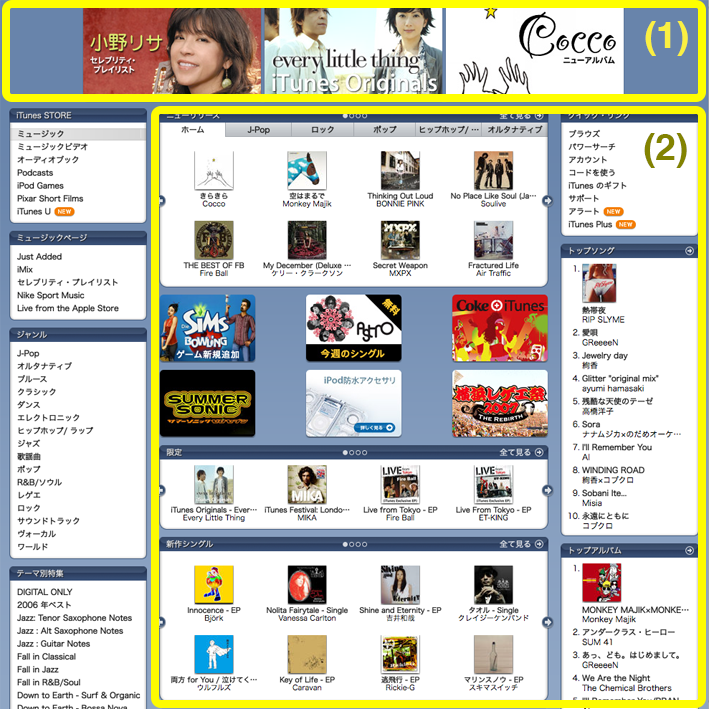
\includegraphics[width=\textwidth]{example1.png}\\
(a)~非個人化 (iTunes Store)
\end{minipage}
\hspace{0.02\fullwidth}
\begin{minipage}{0.45\fullwidth}
\centering
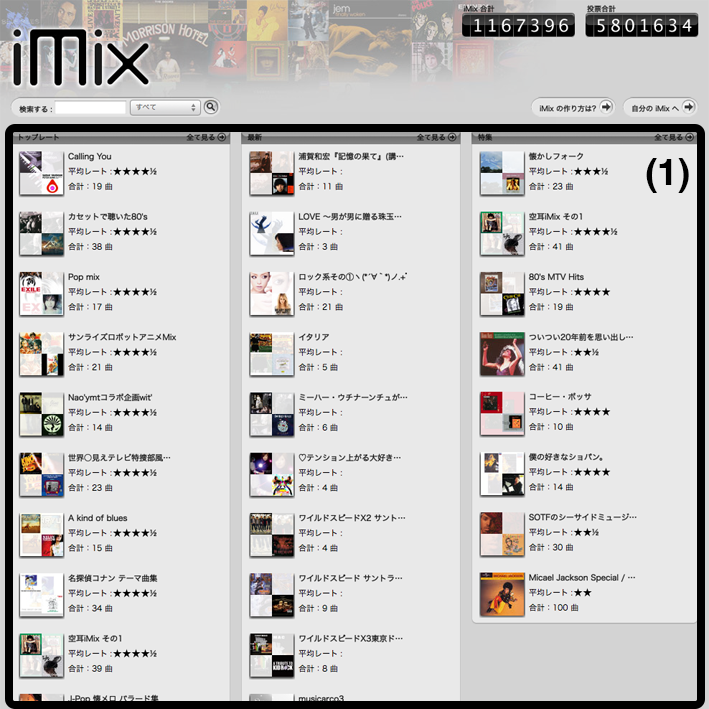
\includegraphics[width=\textwidth]{example2.png}\\
(b)~非個人化 (iTunes Store)
\end{minipage}
\medskip\\
\begin{minipage}[b]{0.45\fullwidth}
\centering
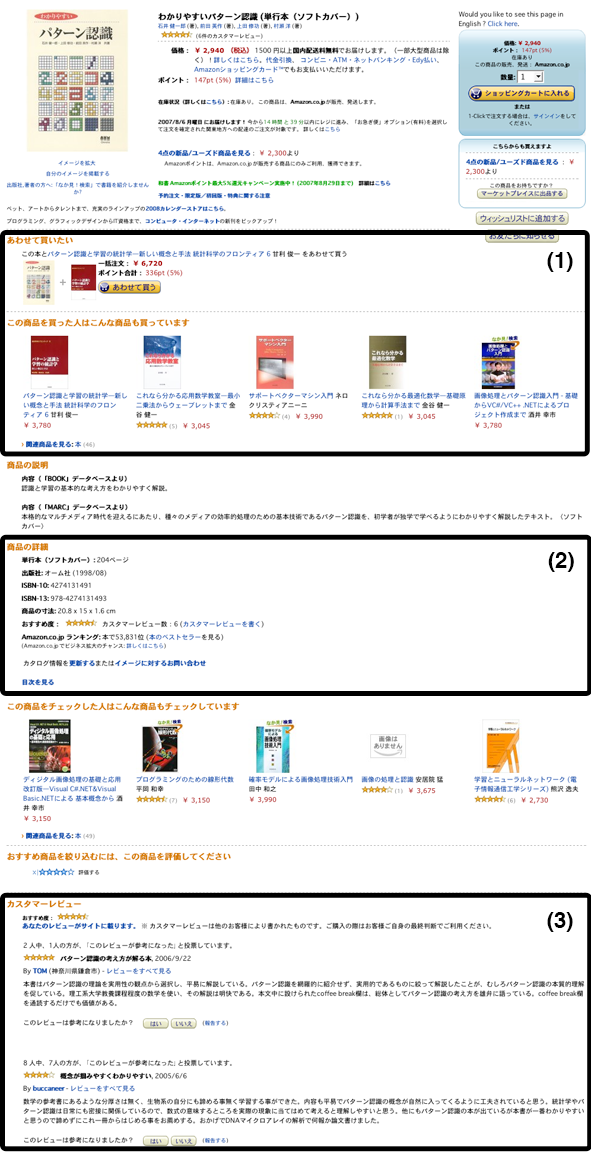
\includegraphics[width=\textwidth]{example56.png}\\
(c)~一時的個人化 (Amazon.co.jp)
\end{minipage}
\hspace{0.02\fullwidth}
\begin{minipage}[b]{0.45\fullwidth}
\centering
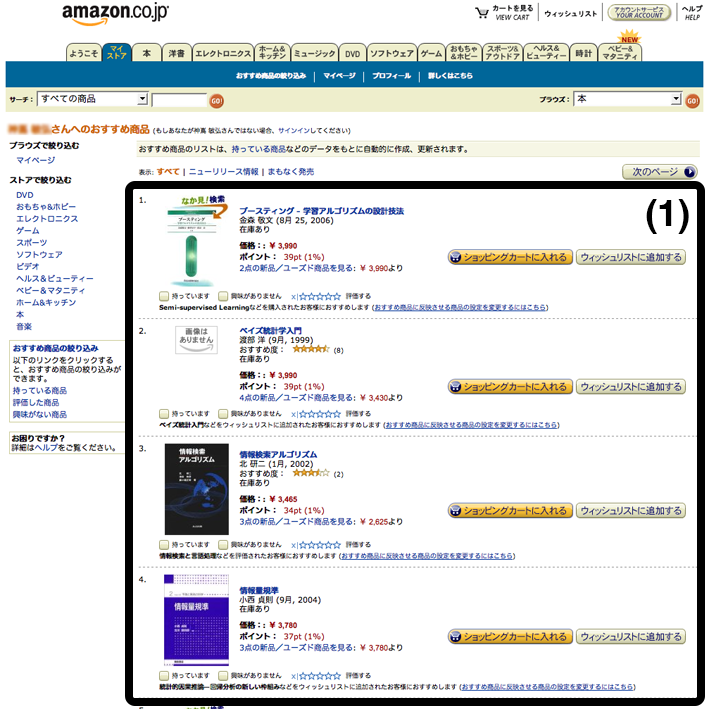
\includegraphics[width=\textwidth]{example4.png}\\
(d)~永続的個人化 (Amazon.co.jp)
\end{minipage}
\bigskip\\
\caption{個人化の度合いの異なる推薦の例}
\label{fig:plevel}
{\footnotesize 図(a),(b),(d) は2007/07/26日に,図(c)は2007/08/04日にスクリーンショットを取得した.}
\end{figure}

\begin{description}[style=nextline]
\item[\term{非個人化}{no personalization}]
全ての利用者について,全く同じ推薦をする場合である.
例えば,編集者による推薦や,売り上げ順位リストなどである.
推薦システムというときは個人化かつ自動化されたものを想定するかもしれないが,こうしたものも広義には含める.
非個人化の推薦の例を図\ref{fig:plevel}(a)と(b)に示す.
図\ref{fig:plevel}(a)中の,(1)は店舗の編集者が手作業で選んだもの,(2)は予約や売り上げの順位リストである.
システム側だけでなく,図\ref{fig:plevel}(b)のように,他の利用者が手作業で作成する推薦リストもある.
\item[\term{一時的個人化}{ephemeral personalization}]
システムを利用する一つのセッションで同じ入力や振る舞いをした利用者には,同じ推薦をする場合である.
一時的個人化の推薦の例を図\ref{fig:plevel}(c)に示す.
この例では,利用者がある本を閲覧するという行動をシステムに対してしたとき,その本に関連する情報を示している.
図中の,(1)はこの本と関連が深い本を推薦し,(2)には,書誌情報や売り上げ順位など,(3)では他の利用者の評価やコメントなど,この本についての関連情報を提示している.
\item[\term{永続的個人化}{persistent personalization}]
たとえ同じ入力や行動をシステムにしている利用者でも,利用者の個人情報や過去の利用履歴に応じて異なる推薦をする場合である.
例えば,過去の購入・利用履歴に基づいて推薦したり,年齢に応じて推薦するアイテムを変えたりする.
永続的個人化の推薦の例である図\ref{fig:plevel}(d)では,この利用者の過去の商品への評価に基づいて,関心があるであろう本を予測し,順位付けして提示している.
\end{description}

\section{推薦システムの運用目的の分類}
\label{sec:systemtarget}

次に,推薦システムを,運用側の目的に基づいて分類する.
文献\cite{dmkd:01:01}では,自動・手動の推薦システムを次の5種類に分
類し,目的に応じて適切に組み合わせて利用すべきと述べている.

\begin{description}[style=nextline]
\item[概要推薦 (broad recommendation)]
これは,全体の統計情報や運用者側の編集者を使う場合である.
全体の統計情報とは「今週の売り上げランキング」や「個々の商品の売り上げ順位」といったもので,編集者による推薦には「評論家が推薦する映画」や「特売品リスト」などがある.
図\ref{fig:plevel}(a)はこうした概要推薦の例である.
こうした概要推薦は,システムを利用し始めたばかりか,ごくまれにしか利用しないような利用者を対象とする.
これらの利用者が,自身の要求との関連性を見いだして,システムの利用を続けてもらえるように,大まかな情報を提供するのが目的である.
よって,積極的に探さなくても見えるように,システムにアクセスしたとき最初に見える場所に配置するべき推薦である.
加えて,利用者が積極的にシステムに働きかけることは期待できないので,非個人化または,アイテムのカテゴリを示す程度の入力に対応した一時的個人化した推薦をすべきである.
\item[利用者評価 (user comments and rating)]
これは,運用側が用意したシステム上で,利用者間での推薦をする場合である.
例えば,読者の批評文や★の数で示した評価レートをつけられるようにし,それらを他の利用者が参照したり,平均評価値などの統計情報を見たりできるようにする.
図\ref{fig:plevel}(b)のような他の利用者による推薦リストや,図\ref{fig:plevel}(c)の(3)のように他の利用者による評価やコメントなどが
この種の推薦の例である.\par
一般に,運用側のシステムが第三者的な立場で推薦しているとは,利用者にはあまり思われない.
それに対し,他の利用者の方がずっと信用され,その推薦も受け入れられやすい.
運用側には,システムに対する利用者の信頼を高めたり,利用頻度を高めたりといった利点がある.
こうした推薦は,運用側の関与は少なく,評価値順のアイテムリストなどの非個人化か,閲覧中のアイテムの評価値やコメントなどの単純な一時的個人化が行われる.
\item[通知サービス (notification service)]
これは,利用者がシステムを操作していないときに,電子メールなどで推薦を配送する場合である.
一つには,過去の購買履歴に基づいて,新規のアイテムの中から推薦リストを生成し,利用者に送付するといった,永続的個人化をするものがある.
また,利用者が予め設定した条件,例えば,ファンである歌手などを設定しておくと,その歌手の新譜の案内が届くという一時的個人化をした推薦もある.
これらの推薦は,システムの再利用を利用者に促すことを目的とする.
\item[関連アイテム推薦 (item-associated recommendation)]
利用者が注目している,例えば,電子商取引サイトで,商品を閲覧しているとか,「買い物かご」にすでに商品を入れている状況を想定する.
このとき,注目しているアイテムの比較候補(例:他メーカーの同等品)を示して,購入の判断を助けたり,購入の決断を促す場合や,補足的な商品などを提示してcross-selling(例:ハンバーガーにポテトなどの関連品を薦めて同時に購入させる)を促す場合がこの種の推薦である.
例としては,図\ref{fig:plevel}(c)の(1)のように閲覧中の商品の関連商品を示すものがある.
注目している商品の情報だけに基づく一時的個人化も,利用者の過去の行動も考慮する永続的個人化も可能である.
\item[緊密な個人化 (deep personalization)]
システムが積極的に利用者の情報を能動的に収集したり,過去の行動の情報を蓄積し,それらに基づいて推薦を行う場合である.
図\ref{fig:plevel}(d)のような,個人向けの推薦リストなどが,この種の推薦に該当する.
利用者がシステムを利用し続けることで蓄積された情報に基づいて,永続的な個人化が可能になる.すると,より適切な推薦ができるようになり,他のシステムとの差別化につながり,利用者の長期間にわたるロイヤリティ構築に役立つ.
だが,一方で,最も実装に困難が伴い,コストも要する.
\end{description}

\section{推薦システムの予測タスクの分類}
\label{sec:recomtask}

推薦システムが達成するタスクに基づく分類を文献\cite{jacm:04:01,jmlr:09:01}に沿って示す.

\begin{description}[style=nextline]
\item[\termmain{適合アイテム発見}{finding some good items}]
このタスクの目的は,利用者が自分の嗜好に適合するものを,何か見つけ出すことである.
利用者が積極的な動機を持って,情報を見つけるために推薦システムを利用するときは,こうした目的になる.\par
例えば,今から食べに行く店を決めるために,レストラン推薦システムを利用することが想定される.
この場合には,予測される評価の高い,比較的少数のものに絞り込んで利用者に提示する.
利用者はこのリストを上位から閲覧することで,自身の決定に必要な情報を知ることができるだろう.
\item[\termmain{評価値予測}{predicting ratings}]
このタスクの目的は利用者がアイテムに付けるであろう評価値を予測することである.
何らかのフォーマットに従ってアイテムが整列されていたり,構造化されている状況を考える.
例えば,新商品を発売日が直近になるように整列したり,カテゴリ別に商品を分類したり,メールや掲示板で記事をスレッド状に表示したりする場合である.
このように整列されたアイテムを,利用者が閲覧しているとする.このとき,閲覧の順序を決めたりとか,どの記事を閲覧するかとかを決めるために,手がかりとなる情報があれば便利である.
そのような情報として,利用者が関心をもつ度合いを,システムは予測して付随的に提示する.
適合アイテム推薦とは違って,利用者には,必ずしも,最終的に意志決定をするような積極的な動機があるとは限らず,また,関
心のあるものを特に選んで表示するといった,アイテムの提示フォーマットを変えるような要求もない.\par
例えば,決まった予定はないが,レストランの紹介Webサイトなどを閲覧しているときなどである.
レストランは,料理の種別や,推薦の度合いは,★の数や,アイコン,グラフなどを対象と共に表示す
ることで利用者に提示する.この推薦情報は,多数のレストランの中から,利用者にとって関心のあるものを絞り込むのに役立つ.
\item[\termmain{適合アイテム列挙}{finding all good items}]
このタスクの目的は,利用者が自分の嗜好に適合するものを網羅的に見つけ出すことである.
これは裏返しに,適合しないものを排除する目的であるともいえる.
例えば,会社の法務部門が関連する特許や判例を検索したり,スパムメールの可能性がないメールだけを閲覧したいといった場合である.
\item[\termmain{効用最適化}{optimizing utility}]
このタスクの目的は,何らかの効用関数を設定し,それを最適化するようなアイテムを見つけることである.
適合するアイテムなら1,それ以外は0という効用関数を考えると,適合アイテム発見はこの効用最適化とみなせるので,適合アイテム発見を一般化したタスクと考えることができる.
例えば,電子商取引サイトで推薦システムによって利益を増やす場合に,元から購入を意図していたアイテムに追加のアイテムを購入させるという組み合わせ販売 (cross-selling) \index{組み合わせ販売}\index{cross-selling}を促進するような効用関数を設定したりする.
\end{description}

\section{推薦システムの利用動機の分類}
\label{sec:usertarget}

文献\cite{sigir:01:01}では,利用者の推薦システムの利用動機の分類を示している.
前者のタイプほど,既知のアイテムに近い推薦することが望まれる.
\begin{description}
 \item[備忘録 (reminder)] 既知のアイテムを思い出させる.
 \item[類似品 (more like this)] 比較などのため既知のアイテムに類似したものを探す.
 \item[新規アイテム (new items)] 自分が確実に好むであろう,未知の新製品を探す.
 \item[視野を広げる (broden my horizon)] 他のジャンルにも自分の関心を広げる.
\end{description}



%!TEX root =  main.tex
%!TEX encoding = UTF-8 Unicode





% privacy
\nocite{kdd:09:01} % 差分プライバシのCF
\nocite{misc:003} % 差分プライバシの基本文献

% social recommendation
\nocite{ec:041}

% popularity bias, diversity
\nocite{misc:011} % PRPの基本文献
\nocite{ej:055}
\nocite{kdd:08:04}
\nocite{recsys:10:01}
\nocite{sigchi:08:01} % bandwagon effect
\nocite{url:005} % LongTailの基本文献

% evaluation
\nocite{etr:008} % ABテストで利用者に悪い影響が残る

% memory-based
\nocite{icdm:07:01} % 近隣法のバイアスとか

% web content optimization
\nocite{jml:02:03} % UCB1
\nocite{icdm:09:01}
\nocite{icml:99:02}
\nocite{www:10:01}

% RBM
\nocite{icml:07:05}

% matrix factorization
\nocite{kdd:08:05}
\nocite{kdd:09:02} % 時間付き
\nocite{kdd:09:03} % テンソル分解,タグ推薦
\nocite{misc:012} % 欠損の考慮
\nocite{url:009} % 確率的勾配降下

% preference elicitation
\nocite{recsys:11:01}


% ===== Back Matter =====
\backmatter
\singlespacing

% ---- Acknowledgements ----
%\medskip
%\noindent\small\textbf{謝辞}:\ 
%みんなありがとう

% ---- Bibliography ----
\bibliographystyle{jsai}
\bibliography{ebib,epublist,emisc,jbib,jpublist,jmisc}

% --- Indexes ---
\printindex

\end{document}
